\section{Data Models and Metadata}

\subsection{Data models}

A dataset definition for clinical research will consist of a number of
different parts, each of which declares a set of related data items.
Typically, this will be a set of data items that would be collected
together: in the completion of a `case report form' in a study, or in
the report of a clinical event.  These parts may be `repeating', in
that there may be more than one form of that type completed, or more
than one event of that type reported upon.  

A data item declaration should explain not only the name under which
values are to be stored, but also the type of those values.  If the
type is numeric, then the unit of measurement should be given.  If the
type is an enumeration, then the intended interpretation of each value
should be explained.  Finally, the parts of the dataset may be
connected or related to one another, and these relationships may have
constrained multiplicities.

It should be clear that a dataset definition can be represented as a
class diagram or object model.  Data items can be introduced as
attributes, parts of the model as classes, and relationships between
classes as associations---complete with multiplicities.  Data types
and enumerations can be used to support attribute declarations, and
hence data item definitions; constraints can be used to express range
restrictions and intended relationships between data items.

Class diagrams can be used also to provide precise definitions for
data sources: existing clinical systems or research databases.  These
systems may be implemented using a combination of technologies but,
assuming that the value of the data justifies the effort required,
precise object models can be created to describe the interfaces that
they might present for data re-use. 

\subsection{Models as metadata}

Having constructed precise object models to describe datasets and data
sources, we can use them as a basis for automated software and data
engineering.  This involves the use of models as metadata in three
respects: for software artefacts that are generated or configured; for
data that these artefacts store or process; and for other models,
capturing relationships between data points declared in different
models, and hence the data stored or processed against them.

For the first of these, we need only maintain the relationship between
the implementation and the model that was used to generate or
configure it.  If the model is stored in a repository or \emph{model
  catalogue} and published, then we have only to create a link between
the implementation and this published instance.  This link may be
created automatically in the case where the model is generated,
partially or completely, from an existing implementation: for example,
from the schema of a relational database.

For the second, a link must be created between each data point, or
collection of data points, and the corresponding declaration in the
data model.  The model catalogue then requires some support for the
language in which the data model is expressed, sufficient to support
the creation and manipulation of links to specific components: in
particular, to specific classes and attributes.  If the data is
acquired or processed using a software implementation for which a data
model has already been registered, then that model may provide a basis
for the automatic creation of a link to the corresponding declaration.

For the third, we need the same ability to create and manipulate links
between components of different models.  Instead of links between
model and implementation, however, we have links representing
different kinds of relationships: provenance and re-use of model
components; versioning of models; and, most importantly,
\emph{semantic relationships} between attributes or
classes---assertions that one attribute or class has the same meaning
or interpretation as another.  This is precisely the information
needed to support automation in data discovery, integration, and
re-use.

\subsection{Models Catalogue}

A software \emph{model} is an abstraction of a software program, which
will be instantiated and run using \emph{real data}, software
modelling is becoming important for a number of reasons, not least
that it enables developers the opportunity to \emph{re-use} code. The
Unified Modelling Language UML \cite{UML} or Ecore \cite{ECORE} ( a
subset of UML) are in widespread use for defining and representing
software \emph{models}. UML and Ecore are defined at a level which is
\emph{more abstract} than the model itself, and one which we term the
\emph{meta-modelling} layer.

Thus there are two things we need to identify and reference in
building the toolkit, firstly does this \emph{concept} \textbf{mean}
the same as that \emph{concept}, and secondly does this \emph{concept}
have the same \emph{representation} as that concept. The way in which
we can match up concepts in software engineering is by associated them
with classes of software objects, and then defining methods which can
reference them.

\subsection{Model Driven Software Development}
......
%%------------NEW STUFF-----------------------%%

%%------------Meta-levels Diagram-----------------------%%


\subsection{Metadata and ISO11179}
ISO11179 is the international standard relating to metadata and in particular metadata registries. It forms the basis of the design of the models catalogue toolkit.

\begin{figure}[here]
	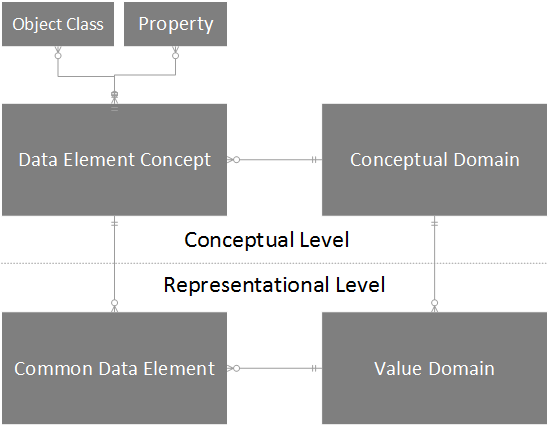
\includegraphics[width=0.48\textwidth,natwidth=610,natheight=642]{BasicISO}
	\caption{Core model for ISO11179 Metadata Registry} 
	\label{fig:basicMDR}
\end{figure}

The ISO11179 standard uses the notion of a \emph{data element concept}, \emph{a data element}, \emph{a value domain}, and a \emph{conceptual domain}. The standard currently confines itself to the detailed level of concepts and data elements and has no notion of collections of data elements or data element concepts, but instead attaches two attributes: an \emph{object class} and a \emph{property} to each data element concept and these attributes allow the data element concept's to be aggregated or classified. This core model of the ISO11179 is illustrated in figure \ref{fig:basicMDR}. The data element concept and conceptual domain entities belong to the \emph{conceptual level}  whilst the common data element and value domain both belong to the \emph{representational level}.


For example an Integer data-type in a programming language may be used to represent inches in a measurement program, it may also be used to count vehicles in a logistics application.  A data element is said to be comprised of a data element concept(DEC) which is its meaning and a value domain(VD) which is its representation.

\begin{table}[h]
	\begin{tabular}{ p{1.8cm} p{2.8cm}  p{3.0cm}  }  % centered columns (2 columns)
		\hline
		Entity & ISO Definition & ISO11179 Implementation Guidelines  \\ 
		\hline
		Data Element Concept(DEC) & An idea that can be represented in the form of a data element, described independently of any particular representation. & A concept that can be represented in the form of a Data Element, described independently of any particular representation.\\
		Common Data Element(CDE) & A unit of data for which the definition, identification, representation, and permissible values are specified by means of a set of attributes. & A unit of data for which the definition, identification, representation and Permissible Values are specified by means of a set of attributes. \\
		Value Domain (VD) & The description of a value meaning. & A description of a Value Meaning. \\
		Conceptual Domain (CD) & A set of valid value meanings, which may be enumerated or expressed via a description.& A set of valid Value Meanings.\\
		\hline
	\end{tabular}
\end{table}

The table lists the definitions of the key entities used in the standard
Conceptual domains comprise sets of value domains, they provide a collection mechanism of \emph{Value Meanings} which provide representation for a particular data element concepts. Data Element Concepts can then be grouped according to their Object Class, or Property, however whilst this works for a system that is focussed entirely on the metadata units, any working software system will need to group the data elements in a structure that is easily transformed into the components such as Classes and Entities that are used in most information systems.   



\subsection{A Language for Data Meta-Modelling }

The ISO11179 specification illustrates different aspects of the standard using UML class diagrams, and we have used these to inform the development of a very simple domain specific language for metadata modelling.The next section gives a description of the language and highlights how it differs from the meta-model outlined in the standard. Probably the key changes are that we have added in containers to handle data element collections, calling these \emph{DataClasses} and to handle collections of these \emph{DataClasses} which we have introduced entities called \emph{DataModels}.

A simplified overview model, without attributes and methods, showing the Ecore model for this DSL is shown in Figure \ref{fig:mcSimplifiedOverview}.
%%------------REDO-----------------------%%
\begin{figure}[here]
	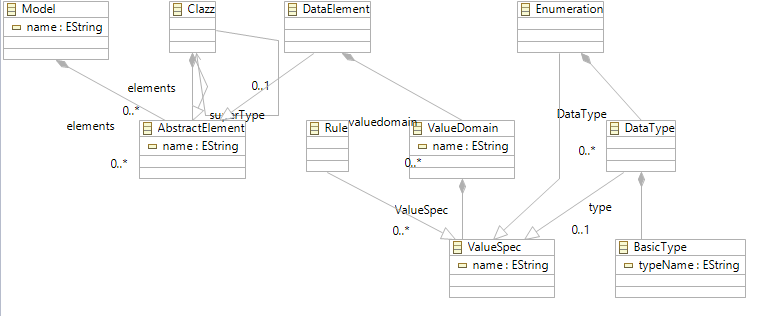
\includegraphics[width=0.5\textwidth,natwidth=610,natheight=642]{ELM_EcoreDiagram}
	\caption{Overview of Metamodel} 
	\label{fig:mcSimplifiedOverview}
\end{figure}

\subsubsection{DataModel}
A datamodel is a grouping or containment entity which groups a set of \emph{DataClasses} together. DataModels can be thought of as datasets, or even database schemas, very often in the medical domain they are defined either by XML Schema definition files, or by equivalent schemas written in Excel. 
DataModels are collections of \emph{ConceptElements} which in turn can be either \emph{Data Elements} or \emph{Classes}. There is no real notion of composition or multiplicity, a instance of a DataModel can contain an instance of a Data Element or not as required by the instance.  DataModels are named, have a description and have a version identity.
\subsubsection{DataClass}
A DataClass is a grouping or collection of \emph{attributes} which can be data elements or classes, the attributes are currently \emph{mandatory}, so that DataClass with 5 attributes must have those 5 attributes instantiated in an instance for it to be considered of that DataClass. A dataclass is named to differentiate it from the term \emph{Class} as used in object oriented programming languages, it captures the structural rather than behavioural aspects of a class.  DataClasses represent \emph{Concepts}, and can be \emph{Generalized} into a hierarchy, giving some of the benefits of inheritance to the language.  
\subsection{Data Elements} 
Data Elements can also represent \emph{Concepts} and are by their nature \emph{atomic}.  Each data element is related to a value domain on a one-to-one basis, and the relationship is a two-way relationship.
\subsection{Value Domain}
A Value Domain is the domain in which the data element is represented, it can consist of one or more \emph{ValueSpecs}.
\subsection{ValueSpec}
A \emph{ValueSpec} can be a simple datatype, an enumeration of datatypes, or a rule - such as a regular expression - which defines the way in which a series of characters is formed into a string attribute. 



The original dataset was collected and managed in Excel, as shown in Figure \ref{fig:excelCOSD}

\begin{figure}[here]
	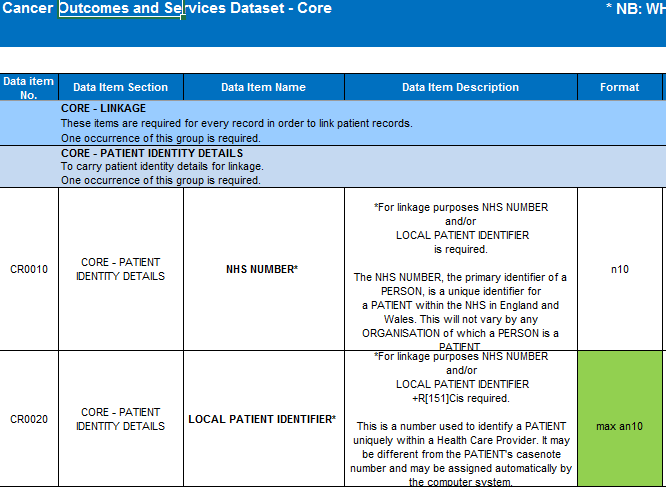
\includegraphics[width=0.5\textwidth,natwidth=610,natheight=642]{COSDExcelS}
	\caption{COSD Datamodel in Excel Format} 
	\label{fig:excelCOSD}
\end{figure}
The DSL is used to represent a model for Cancer data (part of the Cancer Outcomes and Services Dataset ~\cite{COSD}) in Figure \ref{fig:elmcosd}

\begin{figure}[here]
	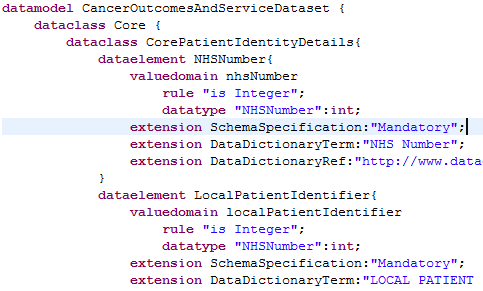
\includegraphics[width=0.5\textwidth,natwidth=610,natheight=642]{MCCOSDModelS}
	\caption{COSD Datamodel in DSL} 
	\label{fig:elmcosd}
\end{figure}



\subsection{Forms and Automatic Software Generation}

%%------------NEW STUFF-----------------------%%

........


